\problem{47}{(สอวน ม.4 2556) เมื่อเริ่มต้น $A$ และ $B$ อยู่ห่างกัน $l$ (ดังรูป) ที่เวลา $t=0$ ทั้ง $A$ และ $B$ เริ่มต้นเคลื่อนที่ไปทางขวา $A$ เคลื่อนที่จากหยุดนิ่งด้วยความเร่งคงที่เท่ากับ $a$ $B$ เคลื่อนที่ด้วยความเร็วคงที่เท่ากับ $v_0$ $A$ ไล่ทัน $B$ ที่เวลา $t$ เท่ากับเท่าใด}
\begin{center}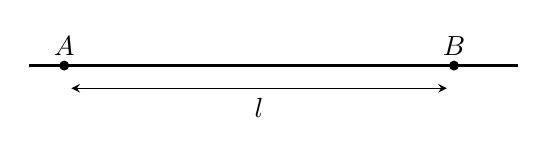
\begin{tikzpicture}[>=stealth,scale=.9]\draw[thick](-.5,0)--(6.4,0);\fill (0,0)circle(2pt) node[above]{$A$};\fill(5.5,0)circle(2pt)node[above]{$B$};\draw[<->](.1,-.32)--(5.4,-.32)node[midway,below]{$l$};\end{tikzpicture}\end{center}
